\documentclass[11pt]{article}
\usepackage[margin=1in]{geometry}
\usepackage{times}
\usepackage{graphicx}
\usepackage{booktabs}
\usepackage{multirow}
\usepackage{amsmath,amssymb}
\usepackage{xcolor}
\usepackage{hyperref}
\usepackage{enumitem}
\usepackage{subcaption}
\usepackage{tikz}
\usetikzlibrary{arrows.meta,positioning,fit}
\hypersetup{colorlinks=true,linkcolor=blue,citecolor=blue,urlcolor=blue}

\title{Compact Theorem Routes for Multimodal Geometry Reasoning\\
\large Selective Exposure of Intermediate Geometry Language}
\author{Anonymous Authors}
\date{June 2026}

\begin{document}
\maketitle

\begin{abstract}
Intermediate geometry language is usually treated as auxiliary context for multimodal large language models (MLLMs): parse the diagram, append symbolic facts, and let the MLLM solve. We argue for a selective-exposure view instead. First, descriptive structure alone is not a reliable intervention. Second, compact theorem routes are a stronger compression layer because they turn a parse into theorem-level actions. Third, the decisive factor is not route format alone, but whether the route is screened and trust-calibrated before exposure. Across Geometry3K, PGPS9K, and GeoQA, GDP-style facts and unfiltered oracle predicates can fail to improve raw image solving. In contrast, theorem routes have real value: on GeoQA271, generated route guidance improves Qwen3-VL-8B from 30.63\% to 38.01\%, and a verified-policy route reaches 40.59\%. A FormalGeo oracle-route check improves 29.00\% to 41.50\%, but we use it only as a qualitative sanity check because FormalGeo and GeoQA differ in difficulty and annotation. The remaining challenge is calibration. On the same GeoQA271 split, verified-policy route remains strongest, while equation and hybrid candidates improve over direct routes. This supports a cascade: screen route first; if route confidence is weak, expose target-bound theorem-equation candidates as a safer selection interface; if confidence remains low, fall back to raw image solving. We also find that compact routes provide inference-time theorem-planning assistance for smaller VLMs: InternVL3-2B rises from 15.75\% to 31.75\%, while gains for stronger 8B models are smaller.
\end{abstract}

\section{Introduction}
Diagram-based geometry reasoning is a compact stress test for multimodal models: the solver must perceive entities, bind labels and quantities, identify applicable theorems, and compute the requested value. Classical neuro-symbolic systems therefore convert diagrams and text into formal language before solving. Inter-GPS parses problems into formal representations for interpretable reasoning \cite{lu2021intergps}; GeoQA studies multimodal numerical geometry reasoning \cite{chen2021geoqa}; FormalGeo organizes conditions, theorem sequences, and verifiable solving traces \cite{zhang2023formalgeo}; and recent parser-centric work such as DFE-GPS and Geoparsing revisits diagram formalization for the MLLM era \cite{zhang2024dfegps,wang2026geoparsing}.

These systems motivate a tempting assumption: exposing intermediate geometry language to an MLLM should improve downstream solving. Our experiments show that the assumption is incomplete. Intermediate language is not passive context; it is an intervention on the model's reasoning trajectory. A correct-looking structured fact can be irrelevant to the target, a theorem route can use a true theorem for the wrong subproblem, and an authoritative route can override a correct visual answer. The central question is therefore not whether to expose intermediate language, but \emph{which mathematical unit should be exposed, and under what reliability condition}.

We study three increasingly action-oriented units: \emph{structured facts}, \emph{compact theorem routes}, and \emph{theorem-equation candidates}. The evidence points to a hierarchy. Structured facts are often insufficient because they describe what is visible but not what should be done. Compact routes are stronger because they compress the parse into theorem-level actions. Theorem-equation candidates are not claimed to dominate verified routes; rather, they are a safer fallback interface when the system cannot confidently verify a route as a sequence.

This paper makes four contributions:
\begin{itemize}[leftmargin=*]
\item \textbf{A counterexample to unconditional structure exposure.} We show that GDP-style automatic structure and even unfiltered oracle predicates can fail to improve Qwen3-VL-8B when appended as ordinary context.
\item \textbf{Compact routes as theorem-level compression and planning assistance.} We show that generated routes can improve downstream MLLM solving by converting a diagram parse into target-oriented theorem actions, with gains on GeoQA and especially large gains for smaller VLMs in a cross-model PGPS9K+Geometry3K test.
\item \textbf{A win--loss view of route reliability.} We evaluate route guidance by pairwise flips against raw image solving, revealing that average gains can hide route-induced corruption.
\item \textbf{A selective-exposure cascade.} We argue that systems should first verify route reliability, then use theorem-equation candidates as a fallback selection interface, and finally hide intermediate language when neither signal is trustworthy.
\end{itemize}

\section{Intermediate Language as a Mathematical Interface}
The contribution is not a new prompt template. The underlying issue is the computational contract between an upstream parser or route generator and the downstream MLLM. Three forms of intermediate language play different mathematical roles:

\begin{itemize}[leftmargin=*]
\item \textbf{Structured facts} describe perceived diagram content: points, lines, angle measures, parallelism, tangency, and other relations.
\item \textbf{Theorem routes} propose a solution path: which geometric principles should be used and in what approximate order.
\item \textbf{Theorem-equation candidates} expose candidate theorem bindings together with executable equation skeletons, forcing the model to select a rule whose preconditions match the target and givens.
\end{itemize}

The candidate interface is closer to theorem application in a formal solver: a theorem can be used only after its preconditions are matched to known facts and its conclusion is connected to the requested target. This perspective explains why a route can be harmful even when it mentions a true theorem. Theorem validity is weaker than target usefulness. However, our same-split results show that a verified route is currently stronger than candidate conversion alone; candidates should therefore be understood as a controlled fallback for uncertain routes, not as a replacement for verification.

\begin{table}[t]
\centering
\caption{A three-level interface hierarchy for intermediate geometry language. The paper's claim is not that later levels replace earlier ones, but that each level fixes a specific failure mode of the previous one.}
\label{tab:interface-hierarchy}
\small
\begin{tabular}{p{0.23\linewidth}p{0.25\linewidth}p{0.25\linewidth}p{0.17\linewidth}}
\toprule
Level & Exposed object & Failure addressed & Primary experiment \\
\midrule
Descriptive facts & parsed points, lines, relations & missing perception, but no action selection & Geometry3K structure tests \\
Compact route & short theorem-action sequence & no theorem planning, but may be target-mismatched & GeoQA271 and cross-model tests \\
Theorem-equation candidates & theorem binding plus equation skeleton & safer fallback when route verification is weak & GeoQA220/271 candidates \\
\bottomrule
\end{tabular}
\end{table}

\begin{figure}[t]
\centering
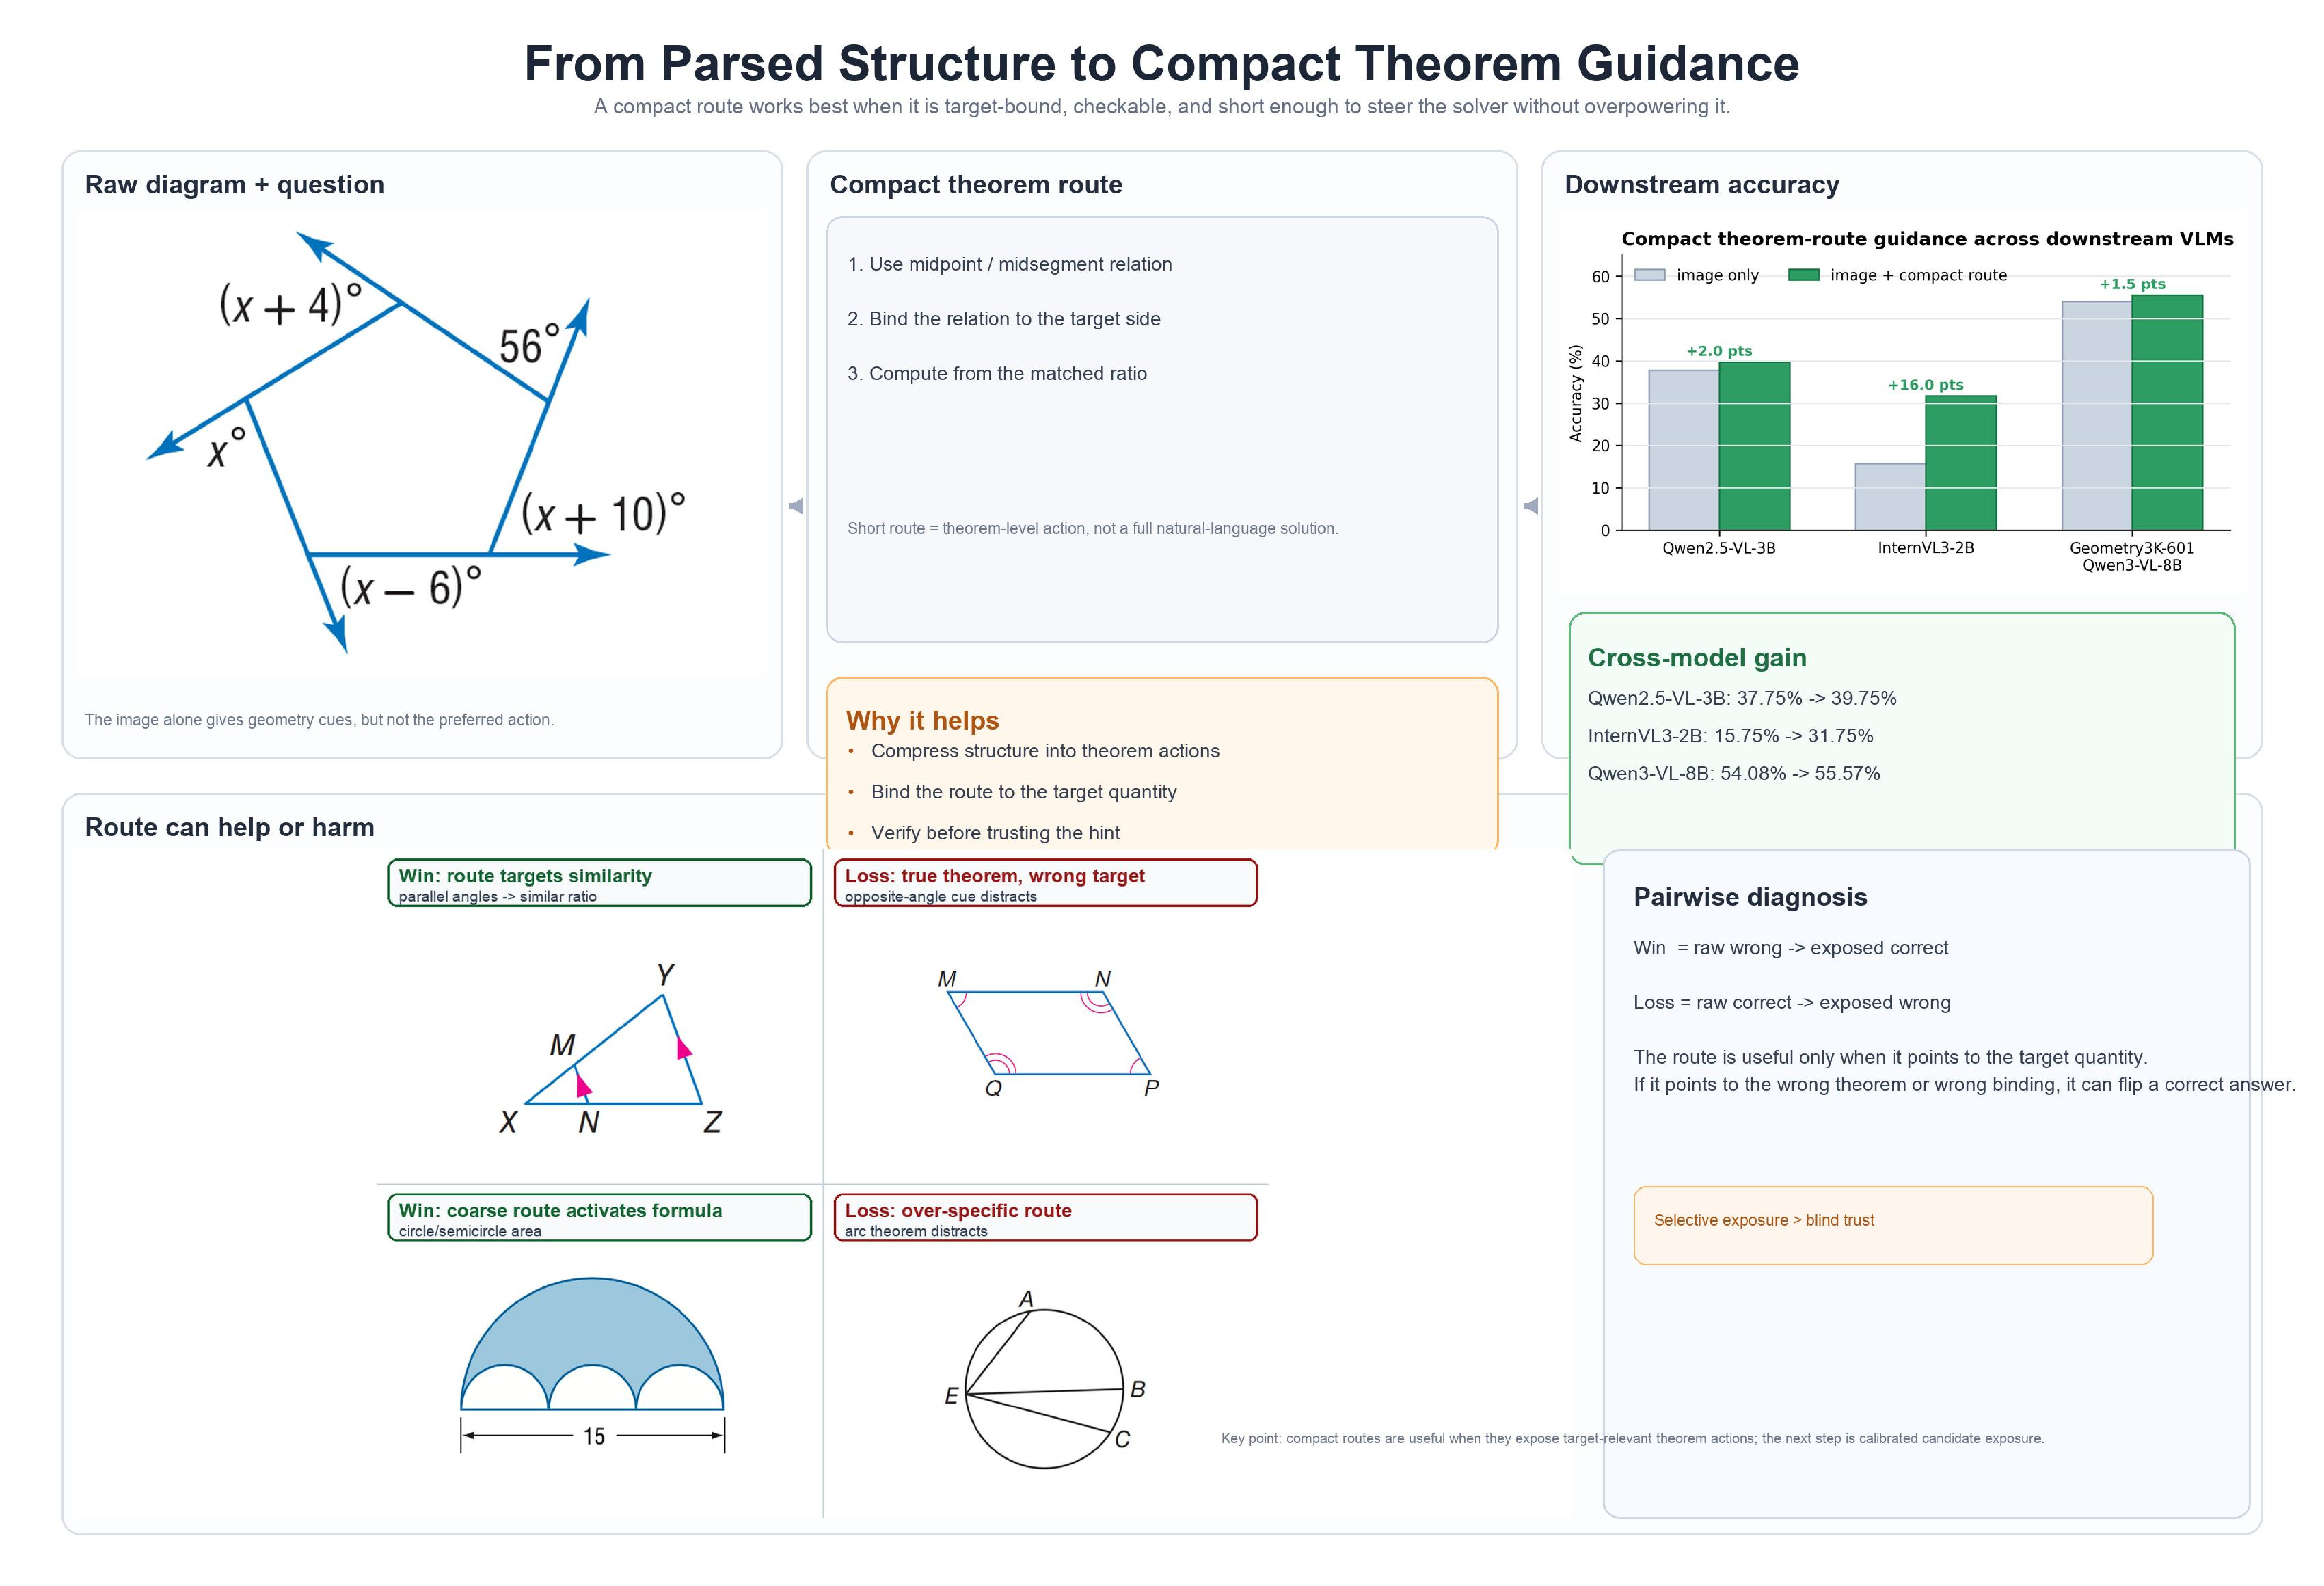
\includegraphics[width=0.98\linewidth]{figures/compact_route_core_result.pdf}
\caption{Core finding and mechanism. A compact route turns parsed geometry into theorem-level actions. In several downstream regimes, image+compact-route input improves raw image solving, but the route must be treated as a target-bound mathematical interface rather than trusted free text.}
\label{fig:compact-route-core}
\end{figure}

\section{Related Work and Gap}
\paragraph{Formal geometry problem solving.}
Formal solvers such as Inter-GPS and FormalGeo emphasize explicit conditions, theorem applications, and symbolic verification \cite{lu2021intergps,zhang2023formalgeo}. This line of work demonstrates that geometry reasoning benefits from structured mathematical state. Our work differs in the role assigned to the formal representation: we do not assume a complete symbolic solver, but study how partial intermediate language should be exposed to an MLLM that still sees the original image.

\paragraph{Geometry diagram parsing and multimodal benchmarks.}
GeoQA, Geometry3K, and MathVista evaluate visual mathematical reasoning under different annotation regimes \cite{chen2021geoqa,lu2021intergps,lu2023mathvista}. Recent diagram formalization work such as DFE-GPS and Geoparsing improves the upstream conversion from diagrams to formal language \cite{zhang2024dfegps,wang2026geoparsing}. These parsers make intermediate-language exposure increasingly practical, but they do not by themselves answer when the downstream MLLM should trust the exposed text. Our experiments show that parser output can help, fail, or harm depending on target binding and exposure policy.

\paragraph{Intermediate reasoning interfaces for MLLMs.}
MLLMs are often improved by adding decompositions, rationales, programs, or symbolic hints. In geometry, however, an intermediate object is not merely a chain of text: it corresponds to theorem preconditions, entity bindings, and equations. This makes blind route following particularly risky. We therefore evaluate intermediate language as a calibrated intervention, using pairwise wins and losses to measure both help and harm.

\begin{table}[t]
\centering
\caption{Positioning relative to representative geometry and visual-math reasoning lines. Prior work improves parsing, formal solving, vision-language pretraining, or instruction tuning; this paper studies when an already generated intermediate representation should be exposed to an MLLM.}
\label{tab:positioning}
\small
\begin{tabular}{lcccc}
\toprule
Line of work & Formal structure & Theorem path & MLLM solver & Exposure calibration \\
\midrule
Inter-GPS / FormalGeo \cite{lu2021intergps,zhang2023formalgeo} & \checkmark & \checkmark & -- & -- \\
GDP / Geoparsing \cite{zhang2022pgdp,wang2026geoparsing} & \checkmark & -- & optional & -- \\
DFE-GPS / GeoX \cite{zhang2024dfegps,xia2025geox} & \checkmark & partial & \checkmark & -- \\
MAVIS / GeoDANO \cite{zhang2025mavis,cho2025geodano} & implicit & implicit & \checkmark & -- \\
\textbf{This paper} & \checkmark & \checkmark & \checkmark & \checkmark \\
\bottomrule
\end{tabular}
\end{table}

\section{Experimental Protocol}
We use Qwen3-VL-8B as the downstream MLLM solver. The main datasets are Geometry3K \cite{lu2021intergps} and GeoQA \cite{chen2021geoqa}; MathVista is used only as an additional visual-mathematical reference point \cite{lu2023mathvista}. GDP-style structure is generated by a parser model in the geometry diagram parsing line of work \cite{wang2026geoparsing}. For route experiments, a saved Qwen3-1.7B LoRA generator maps structured geometry input into a theorem-route style output. The route is then transformed into different downstream interfaces. The route generator is trained on FormalGeo-style route data and is evaluated on held-out or cross-dataset downstream examples; we do not fine-tune it on the GeoQA examples used in the reported GeoQA evaluation.

\paragraph{Split bookkeeping.}
The GeoQA120, GeoQA220, and GeoQA271 subsets are deterministic prefixes of the same filtered GeoQA ordering, restricted to examples with simple numeric answers. Thus GeoQA120 is contained in GeoQA220, and GeoQA220 is contained in GeoQA271. The different sizes reflect different experimental budgets and variants, not different sampling rules. We report them separately because the 271-example run evaluates route policy, the 120-example run tests multiple presentation interfaces cheaply, and the 220-example run evaluates the heavier theorem-equation candidate interfaces. This nesting should be read as a limitation: the cleanest future comparison is to run all interfaces on the same fixed split once compute permits.

We report accuracy and pairwise flips against the raw image baseline. Pairwise wins are cases where raw is wrong and the augmented method is correct. Pairwise losses are cases where raw is correct and the augmented method becomes wrong. This is important because a method can raise average accuracy while still introducing harmful route-induced errors.

Formally, let \(x_i\) denote the image, question, and choices, \(y_i\) the gold answer, and \(z_i\) an exposed intermediate object such as a route or candidate list. Let \(f_0(x_i)\) be the raw-image prediction and \(f_z(x_i,z_i)\) the prediction after exposure. The per-example effect is
\begin{equation}
\Delta_i(z)=
\mathbf{1}[f_z(x_i,z_i)=y_i]-
\mathbf{1}[f_0(x_i)=y_i].
\end{equation}
Then \(\Delta_i=1\) is a win, \(\Delta_i=-1\) is a loss, and the aggregate effect is
\begin{equation}
\mathrm{Gain}(z)=\frac{1}{N}\sum_i \Delta_i(z)=\frac{W(z)-L(z)}{N}.
\end{equation}
This metric makes explicit why a route can be scientifically interesting even when its average gain is small: it may reveal a high-value but poorly calibrated intervention channel.

\paragraph{Verified-policy route.}
The main `verified-policy' setting is a lightweight route-level heuristic, not a learned verifier. In our implementation, we first extract the generated theorem sequence from the route text. Routes with no parseable theorem sequence are rejected. Routes longer than eight steps or containing a theorem name repeated five or more times are treated as low confidence. For the remaining routes, we inspect whether the theorem family matches the target kind and whether the structured parse contains supporting predicates for the route family, such as parallel, right-triangle, or similar-triangle evidence. High-confidence routes are shown to the MLLM together with an explicit use-policy; medium-confidence routes are shown with risk signals; low-confidence routes remain visible only as weak hints that should be secondary to the image; rejected routes are hidden. This is different from \emph{critique-first}, which asks the MLLM to judge the same exposed route after seeing it. The strict-gate ablation below is a separate, more conservative rule set; its lower accuracy shows that hard rejection can discard useful signal.

On GeoQA271, this policy assigns 244 examples to high confidence, 2 to medium confidence, 12 to low confidence, and 13 to reject. Their corresponding verified-policy accuracies are 101/244 (41.39\%), 1/2 (50.00\%), 7/12 (58.33\%), and 1/13 (7.69\%). These subgroup numbers should be read only as an operational audit because the medium and low groups are small; the headline 110/271 result is the weighted accuracy over the full split. The low-confidence setting is not a pure raw fallback in this experiment: the route is still visible as a weak hint, whereas rejected routes are hidden.

\paragraph{Candidate conversion.}
All theorem and equation candidates in the GeoQA experiments are converted from the same generated route source using deterministic rule-based extraction, not a stronger external LLM. We parse theorem calls from the route, deduplicate theorem names in their first-occurrence order, map known theorem names to short natural-language descriptions, and add equation skeletons from a fixed template table, such as triangle angle sum, parallel-angle equality, Pythagorean relation, similar-triangle ratio, or circle-angle equations. Target kind is inferred from question text using keywords for angle, length, area, perimeter, and related quantities. If no usable theorem is parsed, the interface falls back to a ``none of the above / solve from raw image'' option. This design intentionally isolates the effect of exposure format; it does not give candidates extra reasoning ability from another model.

\begin{table}[t]
\centering
\caption{Claim-to-evidence map. Each main claim is tied to the experiment that supports it and to the diagnostic metric used in addition to accuracy.}
\label{tab:claim-evidence}
\small
\begin{tabular}{p{0.34\linewidth}p{0.34\linewidth}p{0.20\linewidth}}
\toprule
Claim & Primary evidence & Diagnostic metric \\
\midrule
Descriptive structure is not automatically helpful. & Geometry3K-300 and Geometry3K-601 trust experiments. & Accuracy and raw-vs-structure flips. \\
Theorem routes can help but may corrupt correct visual answers. & GeoQA271 route experiment and win/loss decomposition. & Pairwise wins, losses, and net gain. \\
Compact routes are useful theorem-level compression. & GeoQA271, Geometry3K-601, and cross-model PGPS9K+Geometry3K validation. & Accuracy, wins/losses, and per-model gains. \\
Selective exposure is a cascade, not a single best format. & GeoQA120/220/271 exposure experiments. & Accuracy, win/loss, and net gain over direct route. \\
\bottomrule
\end{tabular}
\end{table}

\begin{figure}[t]
\centering
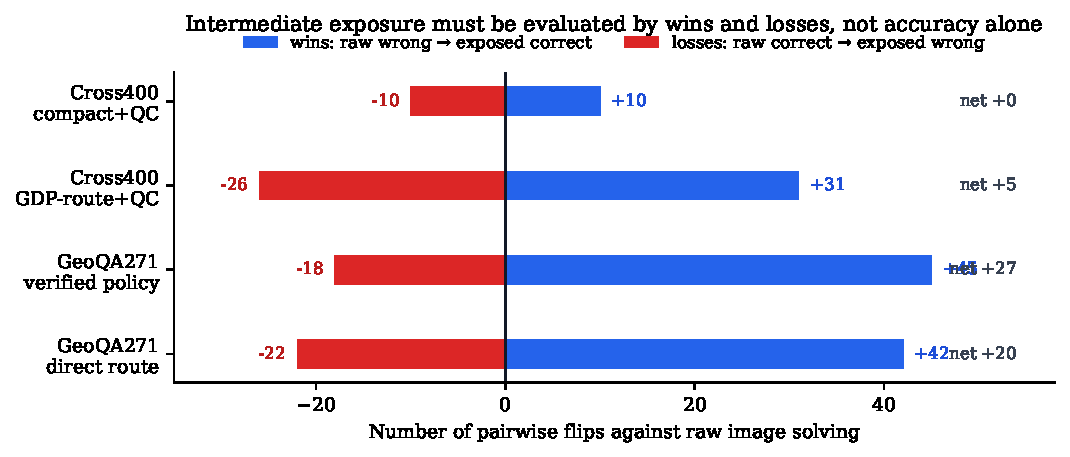
\includegraphics[width=0.88\linewidth]{figures/win_loss_decomposition.pdf}
\caption{Pairwise win/loss decomposition of representative intermediate-exposure variants. Accuracy alone hides whether a method improves by fixing raw errors or by trading those fixes against newly corrupted raw-correct cases.}
\label{fig:win-loss}
\end{figure}

\section{Finding 1: Structure Alone Is Not Enough}
On a Geometry3K-300 subset, simply appending GDP automatic structure does not improve Qwen3-VL. Raw image solving obtains 158/300 correct, while image+GDP obtains 154/300. In pairwise terms, GDP fixes 10 raw errors but breaks 14 raw-correct examples. Oracle-guided construction language is better, reaching 167/300, but this language is not just a flat parse: it is target-conditioned and theorem-aware.

\begin{table}[t]
\centering
\caption{Geometry3K-300 comparison. All structured variants include the original image.}
\label{tab:geometry300}
\small
\begin{tabular}{lccc}
\toprule
Variant & Structure source & Correct / N & Accuracy \\
\midrule
raw & none & 158 / 300 & 52.67\% \\
image+GDP & GDP-4B automatic parse & 154 / 300 & 51.33\% \\
structured facts & Geometry3K oracle predicates & 161 / 300 & 53.67\% \\
construction plan & oracle predicates + theorem cues & 167 / 300 & 55.67\% \\
\bottomrule
\end{tabular}
\end{table}

\begin{figure}[t]
\centering
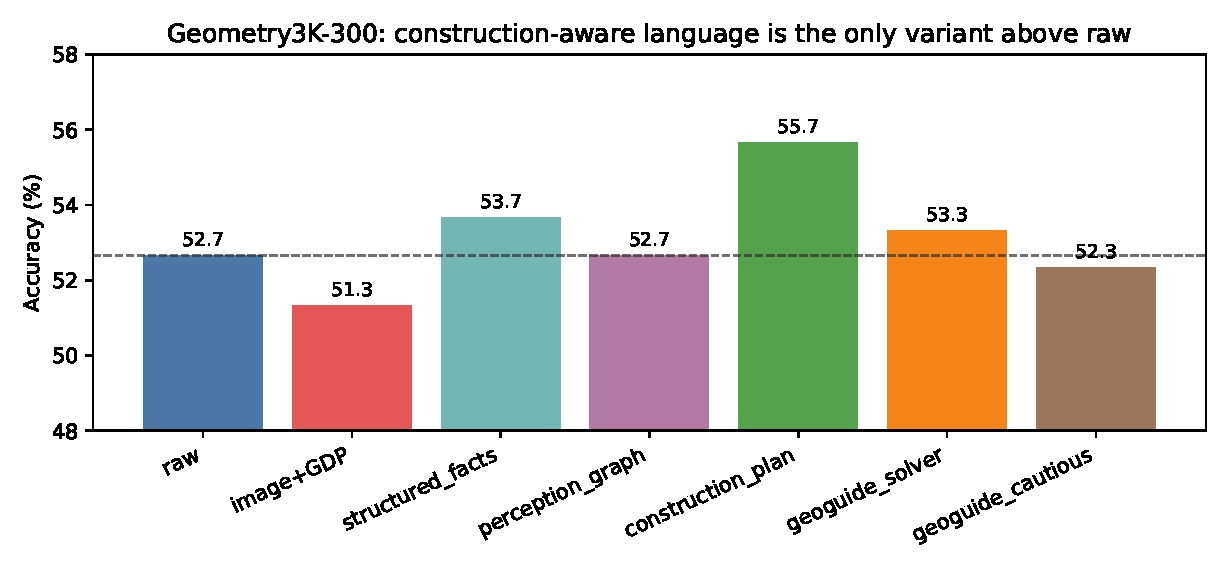
\includegraphics[width=0.82\linewidth]{figures/main_geometry300_accuracy.pdf}
\caption{Structure is not automatically useful. GDP automatic structure is below raw; construction-aware theorem language is stronger.}
\label{fig:geometry300}
\end{figure}

The full Geometry3K-601 trust experiment makes the same point more sharply. Full oracle predicates obtain 318/601, below raw at 325/601. A cautious top-6 version ties raw. This rules out the simplistic explanation that the only bottleneck is missing symbolic facts.

\begin{table}[t]
\centering
\caption{Geometry3K-601 trust experiment. Oracle structure is not a plug-and-play improvement.}
\label{tab:trust601}
\small
\begin{tabular}{lccc}
\toprule
Variant & Correct / N & Accuracy & Interpretation \\
\midrule
raw & 325 / 601 & 54.08\% & image-only baseline \\
oracle\_full & 318 / 601 & 52.91\% & too much unfiltered structure \\
oracle\_topk6\_cautious & 325 / 601 & 54.08\% & filtering recovers raw \\
oracle\_corrupt\_trusted & 314 / 601 & 52.25\% & wrong trusted facts hurt \\
\bottomrule
\end{tabular}
\end{table}

\section{Finding 2: Theorem-Oriented Language Is Useful but Risky}
Theorem routes are more useful than generic structured facts because they are closer to mathematical reasoning. On GeoQA271, generated route guidance improves Qwen3-VL from 83/271 to 103/271. A lightweight verified-policy version reaches 110/271. However, direct routes still produce losses: 22 raw-correct cases become wrong under route guidance.

\begin{table}[t]
\centering
\caption{GeoQA271 route experiment. Routes improve average accuracy but still create route-induced losses.}
\label{tab:geoqa271}
\small
\begin{tabular}{lcccc}
\toprule
Variant & Correct / N & Accuracy & Wins vs raw & Losses vs raw \\
\midrule
image only & 83 / 271 & 30.63\% & -- & -- \\
image + generated route & 103 / 271 & 38.01\% & 42 & 22 \\
image + verified-policy route & 110 / 271 & 40.59\% & 45 & 18 \\
\bottomrule
\end{tabular}
\end{table}

This is the key empirical tension: route language has real mathematical value, but the MLLM can over-follow it. A separate FormalGeo oracle-route check makes the value side of this tension explicit: on 200 FormalGeo examples, dataset-annotated routes improve image-only Qwen3-VL from 58/200 to 83/200. Because FormalGeo differs from GeoQA in problem difficulty, annotation format, and theorem-sequence construction, we treat this only as an auxiliary sanity check and report the full table in Appendix~\ref{app:formalgeo}.

The route generator sometimes repeats a theorem, selects a theorem that is locally plausible but target-irrelevant, or gives a route whose assumptions are not supported by the diagram. A downstream MLLM may then solve the wrong problem confidently.

\begin{figure}[t]
\centering
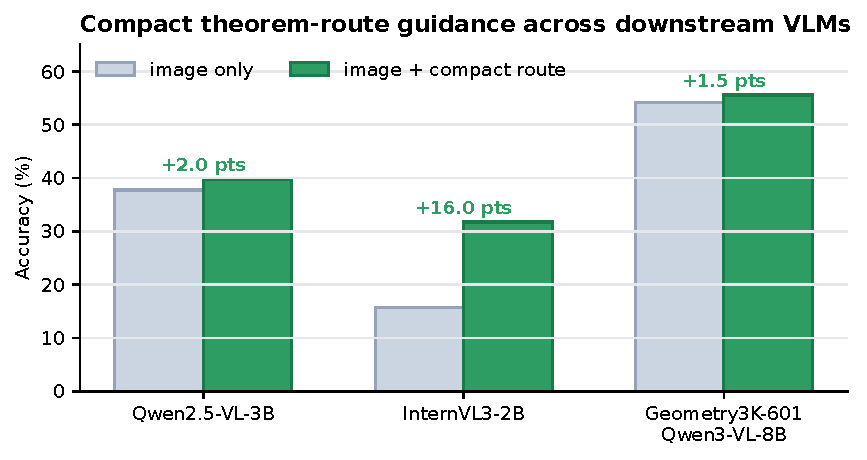
\includegraphics[width=0.86\linewidth]{figures/compact_route_multimodel_accuracy.pdf}
\caption{Compact-route validation across downstream VLMs. The same compact-route channel improves both Qwen2.5-VL-3B and InternVL3-2B on the PGPS9K+Geometry3K split, and is consistent with the earlier Geometry3K-601 Qwen3-VL result. InternVL2.5-2B is excluded because its outputs were not numerically parseable in this run.}
\label{fig:compact-route-multimodel}
\end{figure}

\begin{table}[t]
\centering
\caption{Compact-route gains across downstream VLMs. The compact route is generated upstream and appended to the original image and question. Win/loss is measured against image-only prediction on the same examples.}
\label{tab:compact-route-multimodel}
\small
\begin{tabular}{lcccc}
\toprule
Downstream VLM & Dataset & Image only & Image+compact route & Wins / losses \\
\midrule
Qwen2.5-VL-3B & PGPS9K+Geometry3K-400 & 151 / 400 & 159 / 400 & 26 / 18 \\
InternVL3-2B & PGPS9K+Geometry3K-400 & 63 / 400 & 127 / 400 & 72 / 8 \\
Qwen3-VL-8B & Geometry3K-601 & 325 / 601 & 334 / 601 & 27 / 16 \\
\bottomrule
\end{tabular}
\end{table}

\section{Compact Routes in the Automatic GDP-Route Pipeline}
The previous route experiments show that theorem-oriented language can help, but they do not by themselves establish whether the original automatic pipeline is useful:
\[
\text{image}\rightarrow \text{GDP-4B structure}\rightarrow \text{route generator}\rightarrow \text{MLLM solver}.
\]
We therefore ran this full pipeline on a 400-question mixed split: 200 PGPS9K questions and 200 Geometry3K questions. The same GDP-4B parses are used to generate theorem routes with a fine-tuned Qwen3-1.7B route generator. The downstream solver is Qwen3-VL-8B, and every variant keeps the original image and question.

\begin{table}[t]
\centering
\caption{Cross-dataset GDP-route validation on PGPS9K and Geometry3K. Standard routes with quality control help Qwen3-VL-8B modestly; compact routes are more useful for smaller VLMs in the separate cross-model test.}
\label{tab:gdp-route-cross400}
\small
\begin{tabular}{llccc}
\toprule
Route generator & Dataset & image only & route & route + QC \\
\midrule
\multirow{3}{*}{standard route}
& PGPS9K-200 & 104 / 200 & 101 / 200 & 103 / 200 \\
& Geometry3K-200 & 89 / 200 & 94 / 200 & 95 / 200 \\
& Overall & 193 / 400 & 195 / 400 & \textbf{198 / 400} \\
\midrule
\multirow{3}{*}{compact route}
& PGPS9K-200 & 104 / 200 & 103 / 200 & 105 / 200 \\
& Geometry3K-200 & 89 / 200 & 88 / 200 & 88 / 200 \\
& Overall & 193 / 400 & 191 / 400 & 193 / 400 \\
\bottomrule
\end{tabular}
\end{table}

\begin{figure}[t]
\centering
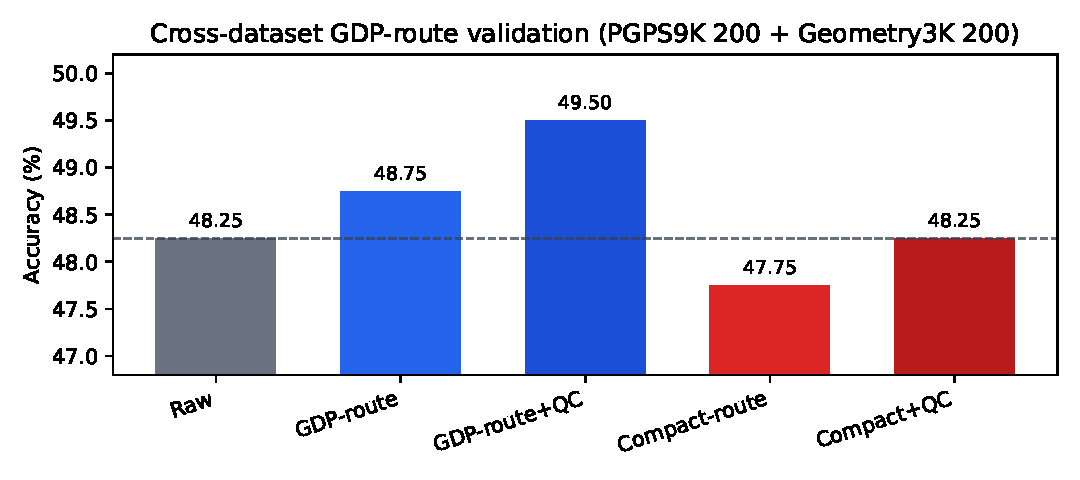
\includegraphics[width=0.86\linewidth]{figures/gdp_route_cross_dataset_400.pdf}
\caption{Cross-dataset GDP-route validation with Qwen3-VL-8B. The standard route with quality control gives a small overall gain; the compact-route result here motivates calibration rather than blind route exposure.}
\label{fig:gdp-route-cross400}
\end{figure}

The cross-model experiment in Figure~\ref{fig:compact-route-multimodel} highlights the most positive regime: smaller VLMs benefit substantially from theorem-level compression. Qwen2.5-VL-3B improves from 37.75\% to 39.75\%, and InternVL3-2B improves from 15.75\% to 31.75\%. The downstream model parameters are not updated; compact routes instead act as a lightweight inference-time planning aid, exposing theorem planning generated upstream to downstream models with weaker internal geometric planning. Table~\ref{tab:gdp-route-cross400} then refines the limitation on a stronger solver. Standard GDP-routes with quality control improve the Qwen3-VL-8B mixed split only from 48.25\% to 49.50\%, with 31 wins and 26 losses against raw. The gain comes mainly from Geometry3K, where route+QC improves 44.5\% to 47.5\%. The compact route in this Qwen3-VL-8B split is not uniformly better. The effect is therefore model-dependent rather than universal, and gains shrink when a stronger VLM already solves many examples from the image.

The correct conclusion is therefore not that compactness alone solves the problem. Compact routes are effective when they expose the missing theorem action, but they still require calibration. In this run, 167/400 compact routes are discarded by simple quality control and 315/400 are marked low-confidence, with an average extracted length of 5.58 theorem steps. This motivates a cascade rather than a single interface: verified routes should be used when confidence is high; when route-level verification is weak, the route should be decomposed into target-bound theorem-equation candidates; when neither route nor candidates are reliable, the system should hide the intermediate language.

\begin{figure}[t]
\centering
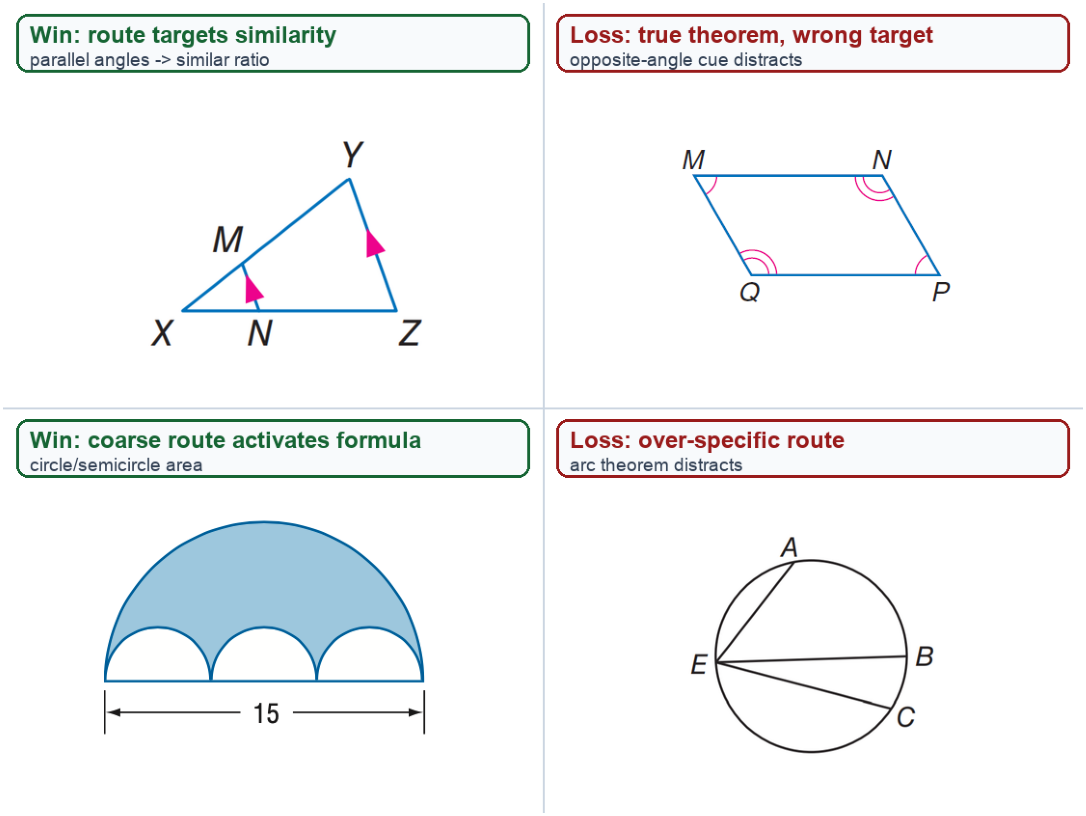
\includegraphics[width=0.88\linewidth]{figures/route_help_harm_cases.pdf}
\caption{Representative route help and harm cases. Helpful routes point the MLLM toward a target-relevant theorem or computation, while harmful routes often mention a true but target-mismatched theorem or add an over-specific cue that distracts from the simpler visual solution.}
\label{fig:route-help-harm}
\end{figure}

Qualitatively, the route-induced errors follow a consistent pattern. In win cases, the route typically names a missing bridge between the target and the givens, such as parallel-angle relations leading to a similarity ratio or a circle-area formula needed for a shaded-region computation. In loss cases, the route is not necessarily nonsensical; it can be target-mismatched: a theorem true in the diagram may not serve the requested quantity. A coarse post-hoc count on GeoQA220 shows that angle problems dominate both direct-route wins and losses (30/32 wins and 14/19 losses), so target type alone is not evidence of binding failure. We use this statistic only to locate where route effects concentrate. Fine-grained labels are still needed to distinguish theorem-name errors, entity-binding errors, arithmetic errors, and visual-attention shifts after seeing route text.

\section{From Theorem Routes to Theorem-Equation Candidates}
Why not simply filter bad routes? A route is a sequence-level object: even after removing very long or obviously repetitive routes, the remaining sequence can still contain a locally valid theorem bound to the wrong target. However, Table~\ref{tab:geoqa271-exposure} shows that verification is more important than format conversion: verified-policy route is stronger than all candidate variants on the same split. The right framing is therefore a cascade. First, verify and expose the route if it is reliable. Second, if route-level confidence is weak, decompose the route into theorem applications and ask whether each application has the right target type, entity binding, and equation consequence. Third, if even candidate-level evidence is weak, return to raw image solving.

We therefore tested a small but informative trust ablation on 120 GeoQA examples. The compared interfaces use the same generated route source but present it differently to Qwen3-VL: direct route execution, critique-before-use prompting, theorem-candidate selection, and a rule-based risk fallback.

\begin{table}[t]
\centering
\caption{GeoQA120 trust ablation. The theorem-candidate interface is the strongest variant in this run.}
\label{tab:geoqa120}
\small
\begin{tabular}{lcccc}
\toprule
Variant & Correct / N & Accuracy & Wins vs raw & Losses vs raw \\
\midrule
image only & 34 / 120 & 28.33\% & -- & -- \\
direct route & 47 / 120 & 39.17\% & 22 & 9 \\
critique-first route & 47 / 120 & 39.17\% & 23 & 10 \\
theorem candidates & 49 / 120 & 40.83\% & 24 & 9 \\
risk fallback & 45 / 120 & 37.50\% & 20 & 9 \\
\bottomrule
\end{tabular}
\end{table}

\begin{figure}[t]
\centering
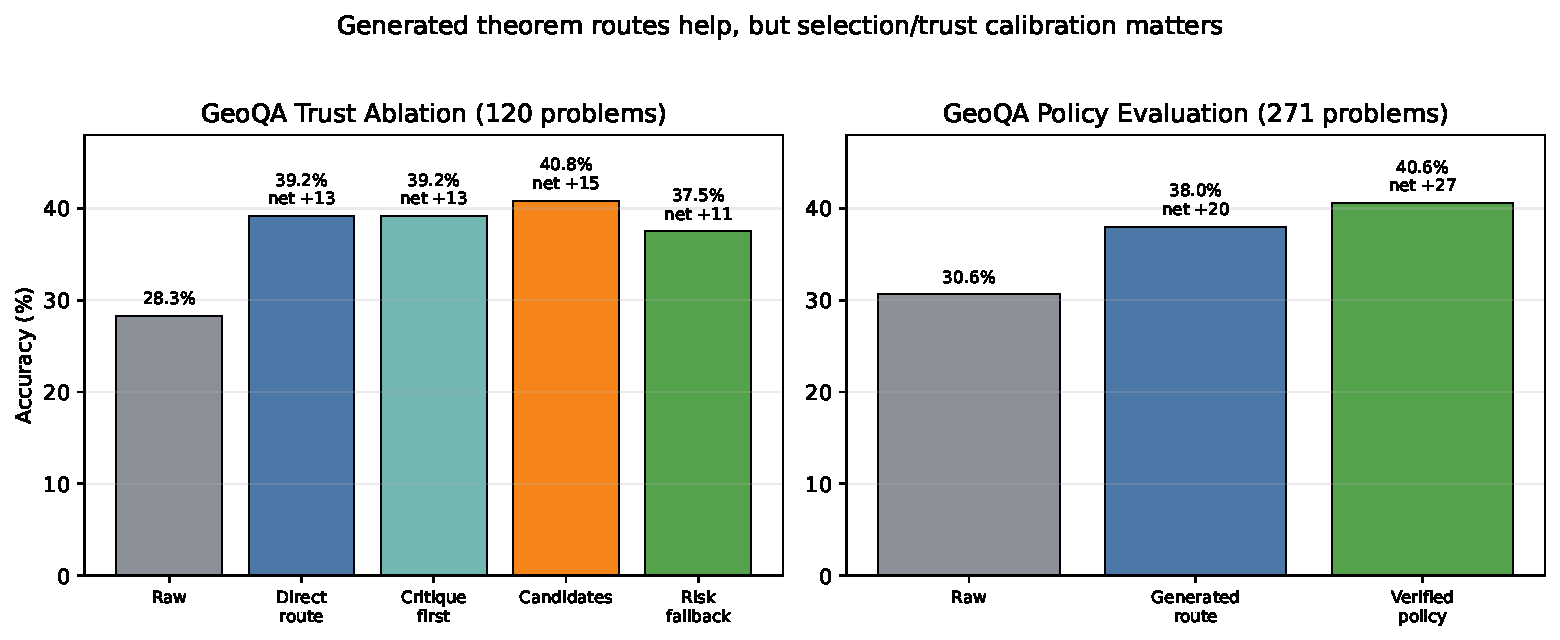
\includegraphics[width=0.88\linewidth]{figures/route_candidate_trust_summary.pdf}
\caption{Route interfaces on GeoQA. Candidate-theorem selection gives the best accuracy and pairwise net in the 120-example trust ablation, while verified policy improves the larger GeoQA271 run.}
\label{fig:route-candidates}
\end{figure}

The 120-problem result suggests that candidate selection can be useful, but it is not the final form of the method. We therefore ran a larger 220-problem GeoQA experiment that compares direct routes, theorem candidates, equation candidates, and a hybrid theorem+equation candidate interface. The result shows that equation-level grounding is more informative than theorem names alone.


\begin{table}[t]
\centering
\caption{GeoQA220 candidate-grounding experiment. Equation candidates and hybrid theorem+equation candidates outperform direct route execution.}
\label{tab:geoqa220-equation}
\small
\begin{tabular}{lccccc}
\toprule
Variant & Correct / N & Accuracy & Wins vs raw & Losses vs raw & Net vs route \\
\midrule
image only & 69 / 220 & 31.36\% & -- & -- & -- \\
route direct & 82 / 220 & 37.27\% & 32 & 19 & -- \\
theorem candidates & 80 / 220 & 36.36\% & 34 & 23 & -2 \\
equation candidates & 84 / 220 & 38.18\% & 32 & 17 & +2 \\
hybrid candidates & \textbf{86 / 220} & \textbf{39.09\%} & \textbf{36} & 19 & \textbf{+4} \\
\bottomrule
\end{tabular}
\end{table}

\begin{figure}[t]
\centering
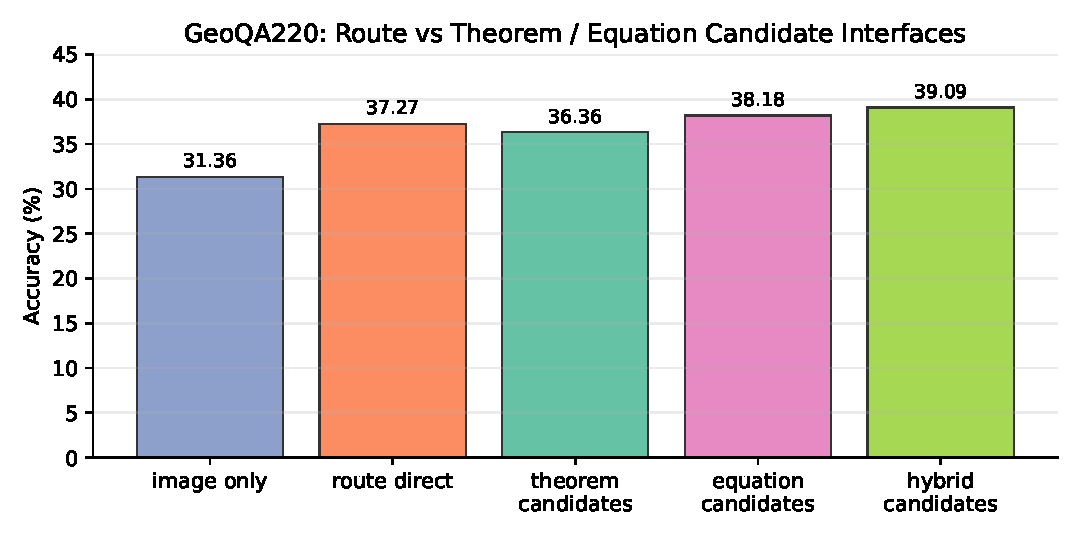
\includegraphics[width=0.86\linewidth]{figures/geoqa220_equation_candidates.pdf}
\caption{GeoQA220 candidate-grounding result. Equation candidates improve over direct routes, and the hybrid theorem+equation interface performs best.}
\label{fig:geoqa220-equation}
\end{figure}


Theorem candidates alone underperform direct routes on the 220-problem run, mainly because they remove some useful sequential information from the route. Equation candidates, however, recover part of this lost information by forcing the model to select a computation skeleton. The hybrid interface is strongest on this 220-example run: it keeps theorem-level semantic guidance while adding equation-level grounding, improving over direct routes by 4 pairwise net cases and over raw by 17 net cases. This supports a refined conclusion: the useful unit is not merely a theorem name, but a target-bound theorem-equation pair.

To avoid comparing variants on different GeoQA subsets, we also reran the exposure variants on the same 271-example split used in Table~\ref{tab:geoqa271}. The result changes the interpretation: reliability control is more important than candidate formatting. Equation and hybrid candidates improve over direct routes, but the verified-policy route is strongest overall. Theorem-only candidates are weaker than direct routes. Candidates are therefore not a magic format by themselves; their role is to make uncertain route information easier to inspect, reject, or partially use.

\begin{table}[t]
\centering
\caption{GeoQA271 same-split exposure comparison and gate ablation. Reliability control is the strongest current intervention: verified-policy route beats all candidate variants, while the strict gate is too conservative. Equation and hybrid candidates still improve over direct route, supporting their role as a fallback interface rather than a replacement for verification.}
\label{tab:geoqa271-exposure}
\small
\begin{tabular}{lccccc}
\toprule
Variant & Correct / N & Accuracy & Wins vs raw & Losses vs raw & Net vs route \\
\midrule
image only & 83 / 271 & 30.63\% & -- & -- & -- \\
route direct & 103 / 271 & 38.01\% & 42 & 22 & -- \\
strict verified route & 86 / 271 & 31.73\% & 26 & 23 & -17 \\
cascade route candidate raw & 91 / 271 & 33.58\% & 30 & 22 & -12 \\
verified-policy route & \textbf{110 / 271} & \textbf{40.59\%} & 45 & 18 & \textbf{+7} \\
theorem candidates & 99 / 271 & 36.53\% & 42 & 26 & -4 \\
equation candidates & 107 / 271 & 39.48\% & 43 & 19 & +4 \\
hybrid candidates & 108 / 271 & 39.85\% & \textbf{46} & 21 & +5 \\
\bottomrule
\end{tabular}
\end{table}

The comparison is still a lower-bound test of the interface, not a full upper-bound result: all GeoQA candidates are converted from the same generated route source by the rule-based extractor described in the experimental protocol, so the candidate pool is constrained by route-generator quality and by the fixed theorem/equation template table. The auxiliary FormalGeo oracle-route result in Appendix~\ref{app:formalgeo} is not a GeoQA upper bound, but it reinforces the qualitative point that reliable theorem routes can be valuable. A stronger evaluation therefore needs oracle candidates derived from annotated theorem sequences on the same target dataset and a learned candidate generator trained directly to emit theorem-equation pairs.

The two gate ablations clarify the tradeoff. The strict verified route is more conservative than verified-policy: it rejects routes longer than six steps, marks any theorem repeated three or more times as risky, requires the theorem family to match the inferred goal type, and checks that parsed facts contain required premise predicates for parallel, perpendicular/right-triangle, or similar-triangle theorems when those theorem families appear. If these strict checks fail, the route is hidden. The cascade variant uses the same strict gate; high-confidence routes are exposed, medium-confidence routes are decomposed into hybrid candidates, and low-confidence routes fall back to raw image solving. This protects against some bad routes but discards too much useful planning signal. Thus the best current policy is not the strictest one; it is the one that exposes route information with calibrated warnings while preserving enough signal for the MLLM to use.

\section{Why Candidate Exposure Is a Safety Interface}
Candidate exposure is not introduced because it outperforms verified routes in the current experiments. It is introduced because direct routes are brittle when route-level verification is unavailable or uncertain. The theorem-equation-candidate interface changes the computational contract between the route generator and the MLLM.

\begin{itemize}[leftmargin=*]
\item \textbf{From assertion to choice.} A route says ``use this theorem.'' A candidate list says ``select the theorem whose preconditions match the target and givens.''
\item \textbf{From sequence following to target binding.} The model must decide whether a theorem solves an angle, a length, a ratio, or an area target.
\item \textbf{From trust to verification.} Wrong candidates can be rejected without rejecting the entire intermediate-language channel.
\item \textbf{From rule names to computation.} Equation candidates force the selected theorem to instantiate a concrete numerical relation, which makes the intermediate language closer to executable mathematics.
\end{itemize}

This framing aligns more closely with formal geometry solvers, where theorem application requires matching preconditions to known facts and binding theorem variables to diagram entities. It also explains why simple critique prompts are weaker: asking the MLLM to ``be careful'' does not provide an explicit alternative action space. Candidate and equation selection do.

\section{Failure Modes and Scope}
The main remaining limitation is that the candidate lists in the GeoQA experiments are converted from generated routes rather than produced by a fully trained theorem-equation selector. This is a deliberate stress test of the exposure interface, but it also means that upstream route quality still constrains the candidate pool. If GDP-style parsing misses a key relation or hallucinates an unsupported relation, the downstream theorem-equation candidates can be incomplete or misleading. Consequently, the present GeoQA numbers should be interpreted as evidence that exposure format and policy can help under a fixed generated-route source, not as the maximum achievable performance of theorem-equation candidates. The FormalGeo oracle-route check suggests that reliable route annotations can be useful, but it does not provide GeoQA oracle theorem-equation candidates. A stronger evaluation needs oracle candidates derived from annotated theorem sequences and a learned candidate generator trained directly to emit theorem-equation pairs.

The results also show that exposure policies must be evaluated across dataset and model regimes. Geometry3K, PGPS9K, and GeoQA differ in annotation style, diagram distribution, and problem type, while Qwen3-VL-8B, Qwen2.5-VL-3B, and InternVL3-2B react differently to route text. Compact routes are most valuable when the downstream model lacks enough internal geometric planning, but even then route-induced losses remain. A deployable system should therefore report performance by dataset, model, target type, and route acceptance status, and should compare generated candidates against oracle theorem labels when such labels are available.

\section{Implication: Target-Binding Verification}
The empirical pattern suggests a concrete architecture: route-first selective exposure with candidate fallback. The input is image, question, choices, and GDP-style structure. The system first scores the generated route as a whole. If route confidence is high, the route is exposed as a strong but still non-oracle hint. If route confidence is medium, the route is decomposed into theorem-equation candidates. If confidence is low, intermediate language is hidden.

A practical candidate-level verifier should check four conditions: whether the theorem matches the target type, whether the bound entities overlap with the question and parsed facts, whether required theorem premises are covered by the parsed fact set, and whether the equation consequence directly solves the requested quantity. We do not assign fixed hand-written weights to these checks. A strict rule-gate ablation on the same GeoQA271 split illustrates why: strict verified route reaches only 86/271 (31.73\%), and a route-candidate-raw cascade reaches 91/271 (33.58\%), both below the lightweight verified-policy route at 110/271 (40.59\%). Coarse rules can reject useful routes and still pass weak ones. The deployable cascade should therefore combine these checks with a learned target-binding verifier:

\begin{itemize}[leftmargin=*]
\item high route confidence: expose verified route as a strong hint;
\item medium route confidence: expose theorem-equation candidates and ask the MLLM to choose;
\item low confidence: hide the intermediate language and fall back to raw image solving.
\end{itemize}

The next model-building step is to train and evaluate this verifier on pairwise labels: raw wrong and route correct implies \textsc{use-route}, while raw correct and route wrong implies \textsc{reject-route}. The important principle is now sharper than ``use candidates'': intermediate geometry language is useful when it is theoremized, verified, and selectively exposed, with candidate selection serving as a safety interface when route-level verification is insufficient.

\section{Conclusion}
Our main conclusion is not that structured language fails, nor that route guidance always helps. The evidence supports a sharper claim: intermediate geometry language becomes useful when it moves from descriptive structure to compact theorem-level action, but action-level language must be selectively exposed. Compact routes improve GeoQA and can strongly help smaller VLMs as inference-time theorem-planning assistance. Their limitation is reliability, not usefulness. The practical implication is a cascade: verify route first; if verification is weak, convert route information into target-bound theorem-equation candidates; if confidence remains low, hide the intermediate language and rely on raw image solving.

\appendix
\section{Auxiliary FormalGeo Oracle-Route Sanity Check}
\label{app:formalgeo}

Table~\ref{tab:formalgeo-oracle-route} reports the FormalGeo oracle-route check mentioned in the main text. It is included as a qualitative sanity check rather than a direct comparison with GeoQA because FormalGeo has different difficulty, annotation format, and theorem-sequence construction.

\begin{table}[h]
\centering
\caption{FormalGeo oracle-route qualitative sanity check.}
\label{tab:formalgeo-oracle-route}
\small
\begin{tabular}{lcccc}
\toprule
Variant & Correct / N & Accuracy & Wins vs raw & Losses vs raw \\
\midrule
image only & 58 / 200 & 29.00\% & -- & -- \\
image + oracle theorem route & 83 / 200 & 41.50\% & 32 & 7 \\
\bottomrule
\end{tabular}
\end{table}

\bibliographystyle{unsrt}
\bibliography{refs}

\end{document}
